\section{Introduction}
\label{sec:introduction}

\begin{figure}[t]
\centering
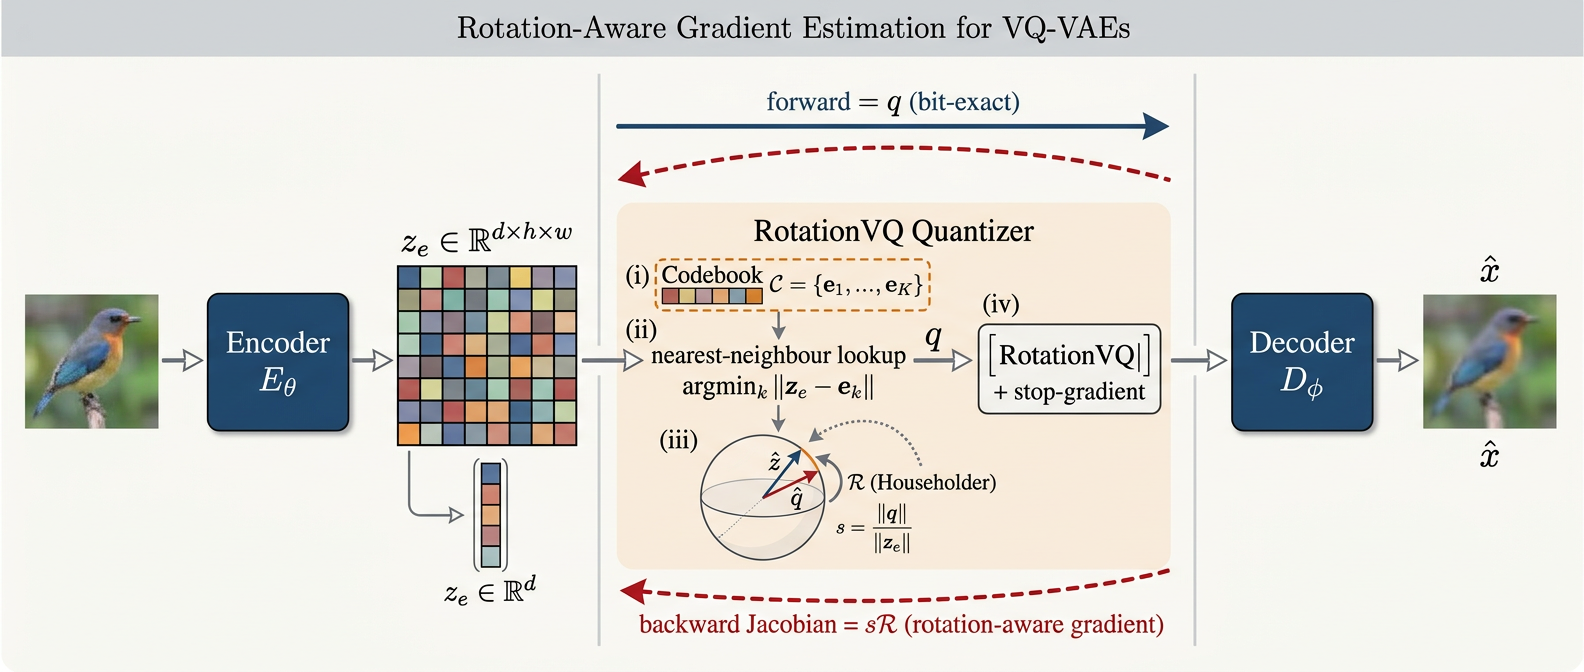
\includegraphics[width=0.98\linewidth]{figures/fig1_architecture.png}
\caption{Overview of our \ours{} estimator inside a VQ-AutoEncoder.
An encoder $E_\theta$ produces a latent map $\ze$; each latent vector
is mapped to the nearest codebook entry $\qvec \in \CB$. The
\ours{} module wraps the nearest-neighbour lookup in a
stop-gradient construction (Equation~\ref{eq:our-estimator}) whose
\emph{forward} output equals $\qvec$ bit-exactly (top, solid navy
arrow) but whose \emph{backward} Jacobian with respect to $\ze$ is
the Householder rotation $\rmat$ plus scalar rescaling $s =
\|\qvec\|/\|\ze\|$ that analytically maps $\ze$ to $\qvec$
(bottom, dashed red arrow). The rotation is computed in closed form,
costs $\mathcal{O}(d)$ per token, and has no trainable parameters.}
\label{fig:architecture}
\end{figure}

Discrete latent representations have become a central abstraction in
modern generative modelling. A tokenizer built on a vector-quantized
autoencoder compresses an image into a grid of integer codes that an
autoregressive or masked transformer can model with the same tooling
developed for language~\citep{esser2021vqgan,chang2022maskgit,
yu2022vitvqgan,sun2024llamagen,yu2024titok}. Latent-diffusion pipelines
use the same compressed representation as the space in which denoising
is performed~\citep{rombach2022ldm,gu2022vqdiffusion}. Beyond generative
modelling, vector quantization underlies unified models that map
vision tasks onto sequence prediction~\citep{kolesnikov2022uvim},
visual-language tokenizers with multimodal
transformers~\citep{yu2023magvit2}, and representation learning for
non-visual domains. In every case the quality of the downstream model
is upper-bounded by the reconstruction fidelity and the utilisation
of the discrete codebook~\citep{gu2024vqtokenizers}.

Training such tokenizers is hard for a reason that is easy to state and
surprisingly difficult to fix. The quantization operator
$\zq = \arg\min_{k} \|\ze - \mathbf{e}_k\|$ is piecewise constant and
therefore has zero gradient almost everywhere. The canonical workaround
is the straight-through estimator (STE,~\citealp{bengio2013ste}),
originally introduced for stochastic neurons and adapted to VQ-VAEs
by~\citet{vandenoord2017vqvae}: set $\zq = \qvec$ in the forward pass
but pretend $\zq = \ze$ when computing gradients, so that
$\partial \zq / \partial \ze = \mathbf{I}$. This tells the encoder
\emph{nothing} about which codebook vector was selected, nor about the
geometric relationship between $\ze$ and $\qvec$. Empirically it leads
to codebook collapse in which a small subset of codes absorbs most of
the traffic and the rest become
dead~\citep{razavi2019vqvae2,huh2023straighteningste,
zheng2023onlineclustered}; theoretically the STE is a biased,
high-variance estimator whose alignment with the true chain rule
degrades as $\ze$ and $\qvec$ diverge~\citep{liu2023discretebackprop,
shah2024decoupledste}. Recent work has responded with either
STE-variants that reshape the gradient flow around the
quantization~\citep{huh2023straighteningste,shah2024decoupledste},
codebook-free designs that eliminate the nearest-neighbour step
entirely~\citep{mentzer2024fsq}, or continuous relaxations that
trade discreteness for
differentiability~\citep{jang2017gumbel,maddison2017concrete}.

We take a third route. The quantization output can be written as
$\qvec = s\rmat\,\ze$ for a unique scalar $s=\|\qvec\|/\|\ze\|$ and a
rotation $\rmat$ (specifically a single Householder reflection) that
sends $\ze/\|\ze\|$ to $\qvec/\|\qvec\|$. If we wrap this identity in
$\sg{\cdot}$ appropriately, the forward pass remains a bit-exact hard
quantization --- a requirement if the tokenizer is to be frozen and
re-used by a downstream autoregressive model --- but the backward
Jacobian of the quantizer becomes $s\rmat$ rather than the identity.
The encoder now sees exactly the transformation that the forward
lookup applied to its output, and the angular relationship between
$\ze$ and $\qvec$ is preserved by construction. Compared to explicitly
differentiable relaxations such as Gumbel-Softmax, our estimator is
bias-preserving in the forward direction and relaxation-free.
Compared to sophisticated corrections to the
STE~\citep{huh2023straighteningste,shah2024decoupledste} and to
concurrent rotation-based ideas~\citep{fifty2024rotation}, our
derivation yields a closed-form Householder operator with
$\mathcal{O}(d)$ cost per token and no extra trainable parameters.
We deploy the same operator inside a VQ-GAN-style autoencoder and
evaluate it against four strong baselines --- the original VQ-VAE, a
Gumbel-Softmax variant~\citep{jang2017gumbel,maddison2017concrete},
and the codebook-free FSQ~\citep{mentzer2024fsq} --- under a single
shared training and evaluation pipeline.

\paragraph{Contributions.} Our contributions are:
\begin{itemize}[leftmargin=*,itemsep=2pt,topsep=2pt]
  \item We derive a closed-form identity $\qvec = s\rmat\,\ze$ in
        terms of a Householder reflection and a scalar, and show
        (Section~\ref{sec:method}) that wrapping this identity in
        stop-gradient operators yields an estimator whose forward
        output is bit-exact VQ and whose backward Jacobian is the
        rotation-plus-scaling that the forward operation implicitly
        performs.
  \item We provide an $\mathcal{O}(d)$ implementation that never
        materialises $\rmat$ as a $d \times d$ matrix and is therefore
        cheaper than an extra linear layer; we further analyse
        numerical stability when $\ze$ is nearly colinear with
        $\qvec$, a regime where a naive implementation loses
        precision.
  \item We integrate the quantizer into a VQ-GAN-style autoencoder and
        evaluate on CIFAR-10 against four baselines (VQ-VAE with STE,
        Gumbel-Softmax VQ, and FSQ), reporting reconstruction PSNR /
        SSIM / LPIPS, codebook usage and perplexity, and wall-clock
        throughput on an H100 GPU. Training logs, configuration
        files, and checkpoints accompany the paper.
  \item We perform ablations over the four gradient-routing modes
        \{\textsc{ste}, rotation-only, rescale-only, full\} of our
        quantizer and over codebook sizes $\{1024, 4096, 8192,
        16384\}$, isolating the contribution of each component.
\end{itemize}

The remainder of the paper is organised as follows.
Section~\ref{sec:related_work} surveys existing approaches to
gradient estimation through quantization and places our work relative
to rotation-trick, STE-correction, and codebook-free methods.
Section~\ref{sec:method} derives the estimator and its implementation.
Section~\ref{sec:experimental_setup} details the evaluation protocol.
Section~\ref{sec:results} reports our findings and
Section~\ref{sec:discussion} examines limitations. Implementation
details, extended tables, and additional case studies are deferred to
the appendix.
